% AEGIS Framework Architecture Diagram — Standalone compilable TikZ
% Fits IEEE two-column span (~7.16in) or single-column (~3.5in) when scaled
\documentclass[11pt,border=4pt]{standalone}
\usepackage[T1]{fontenc}
\usepackage{lmodern}
\usepackage{amsmath,amssymb}
\usepackage{tikz}
\usetikzlibrary{
  positioning,
  arrows.meta,
  calc,
  fit,
  backgrounds,
  decorations.pathreplacing,
  shapes.geometric,
  shadows.blur,
  patterns
}
\usepackage{xcolor}

% ── Color palette ──────────────────────────────────────────────────
\definecolor{inputbg}{HTML}{FAFAFA}
\definecolor{layer1}{HTML}{D6EAF8}
\definecolor{layer1dark}{HTML}{85C1E9}
\definecolor{layer2}{HTML}{D5F5E3}
\definecolor{layer2dark}{HTML}{82E0AA}
\definecolor{layer3}{HTML}{FDEBD0}
\definecolor{layer3dark}{HTML}{F0B27A}
\definecolor{layer4}{HTML}{E8DAEF}
\definecolor{layer4dark}{HTML}{BB8FCE}
\definecolor{appbg}{HTML}{F2F3F4}
\definecolor{appborder}{HTML}{BDC3C7}
\definecolor{complexgray}{HTML}{7F8C8D}
\definecolor{routerbg}{HTML}{F8F9F9}
\definecolor{accentorange}{HTML}{E67E22}
\definecolor{glowcolor}{HTML}{F39C12}

\pagestyle{empty}

% ── LaTeX command for complexity annotations inside node text ──────
\newcommand{\cpx}[1]{{\sffamily\tiny\color{complexgray}#1}}

\begin{document}
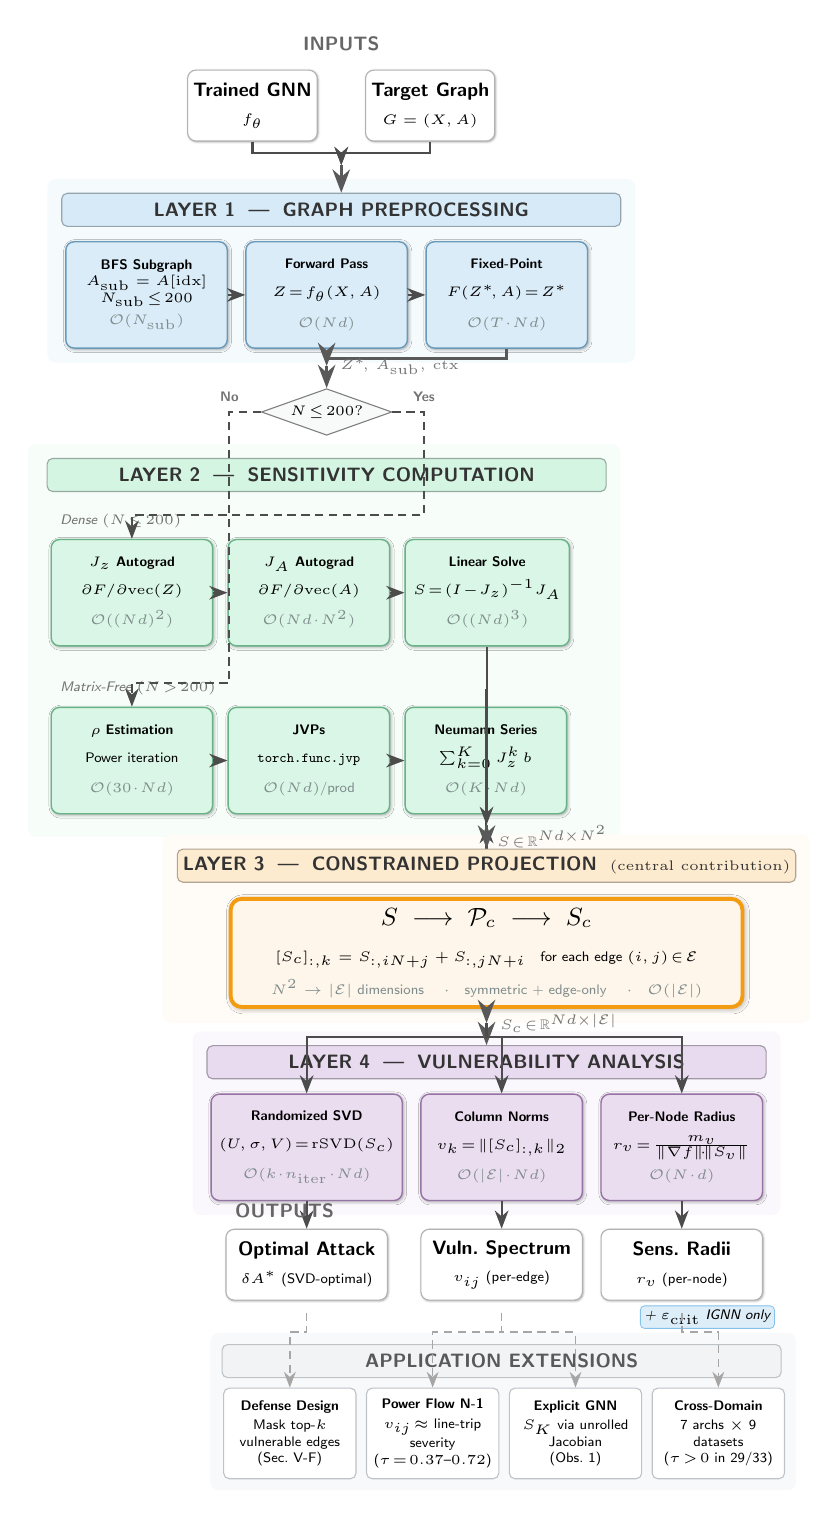
\begin{tikzpicture}[
  % ── Global styles ────────────────────────────────────────────────
  >=Stealth,
  font=\sffamily\small,
  node distance=0.25cm,
  % Processing block
  block/.style={
    rectangle, rounded corners=3pt,
    draw=#1!80!black, line width=0.5pt,
    fill=#1!30, minimum width=2.05cm, minimum height=1.35cm,
    inner sep=3pt, align=center,
    blur shadow={shadow blur steps=4, shadow xshift=0.4pt,
                 shadow yshift=-0.4pt, shadow blur radius=1.2pt}
  },
  block/.default=layer1dark,
  % Layer banner
  banner/.style={
    rectangle, rounded corners=2pt,
    fill=#1, draw=#1!70!black, line width=0.4pt,
    minimum height=0.42cm, inner sep=2pt,
    font=\sffamily\scriptsize\bfseries, text=black!80
  },
  % Input / Output box
  iobox/.style={
    rectangle, rounded corners=3pt,
    draw=black!30, fill=white,
    minimum width=1.6cm, minimum height=0.9cm,
    inner sep=2pt, align=center,
    blur shadow={shadow blur steps=3, shadow xshift=0.3pt,
                 shadow yshift=-0.3pt, shadow blur radius=0.8pt}
  },
  % App extension block
  appblock/.style={
    rectangle, rounded corners=2pt,
    draw=appborder, fill=white,
    minimum width=1.68cm, minimum height=1.15cm,
    inner sep=2pt, align=center,
    font=\sffamily\tiny
  },
  % Arrow styles
  flowarrow/.style={->, thick, color=black!70},
  layerarrow/.style={->, line width=1.2pt, color=black!65},
  % Equation / complexity styles
  eqtext/.style={font=\rmfamily\tiny, text=black!85},
  cpxtext/.style={font=\sffamily\tiny, text=complexgray},
  % Badge
  badge/.style={
    rectangle, rounded corners=1.5pt,
    fill=layer1!80, draw=layer1dark, line width=0.3pt,
    font=\sffamily\tiny\itshape, inner sep=1.5pt
  },
  % Router diamond
  router/.style={
    diamond, draw=black!50, fill=routerbg,
    inner sep=1pt, font=\sffamily\tiny, aspect=2.8,
    minimum width=1.4cm
  },
  % Path container
  pathbox/.style={
    rectangle, rounded corners=3pt,
    draw=#1!60!black, line width=0.5pt, dashed,
    fill=#1!8, inner sep=4pt
  }
]

% ════════════════════════════════════════════════════════════════════
%  TOTAL CANVAS WIDTH  ~  7.1 cm  (fits \columnwidth when scaled)
% ════════════════════════════════════════════════════════════════════

% ── INPUTS ─────────────────────────────────────────────────────────
\node[iobox] (gnn) {%
  {\scriptsize\bfseries Trained GNN}\\[-1pt]
  {\tiny $f_\theta$}};
\node[iobox, right=0.6cm of gnn] (graph) {%
  {\scriptsize\bfseries Target Graph}\\[-1pt]
  {\tiny $G=(X,A)$}};

% Input label
\node[above=0.12cm of $(gnn.north)!0.5!(graph.north)$,
      font=\sffamily\scriptsize\bfseries, text=black!60] (inlabel) {INPUTS};

% Merge point
\coordinate (merge) at ($(gnn.south)!0.5!(graph.south)+(0,-0.3)$);
\draw[flowarrow] (gnn.south) -- ++(0,-0.15) -| (merge);
\draw[flowarrow] (graph.south) -- ++(0,-0.15) -| (merge);

% ── LAYER 1 BANNER ────────────────────────────────────────────────
\node[banner=layer1, minimum width=7.1cm,
      below=0.35cm of merge] (L1ban)
  {LAYER 1\; ---\; GRAPH PREPROCESSING};

% Layer 1 blocks
\node[block=layer1dark, below=0.18cm of L1ban.south west,
      anchor=north west, xshift=0.05cm] (bfs) {%
  {\tiny\bfseries BFS Subgraph}\\[-1pt]
  \parbox{1.8cm}{\centering\tiny $A_{\mathrm{sub}}=A[\mathrm{idx}]$\\$N_{\mathrm{sub}}\!\le\!200$}\\[-1pt]
  \cpx{$\mathcal{O}(N_{\mathrm{sub}})$}};

\node[block=layer1dark, right=0.22cm of bfs] (fwd) {%
  {\tiny\bfseries Forward Pass}\\[-1pt]
  {\tiny $Z\!=\!f_\theta(X,A)$}\\[0pt]
  \cpx{$\mathcal{O}(N d)$}};

\node[block=layer1dark, right=0.22cm of fwd] (fp) {%
  {\tiny\bfseries Fixed-Point}\\[-1pt]
  {\tiny $F(Z^*\!,A)\!=\!Z^*$}\\[0pt]
  \cpx{$\mathcal{O}(T\!\cdot\!N d)$}};

% Arrows within layer 1
\draw[flowarrow] (bfs.east) -- (fwd.west);
\draw[flowarrow] (fwd.east) -- (fp.west);

% Arrow from merge to layer 1
\draw[layerarrow] (merge) -- (L1ban.north);

% ── INTERFACE / ROUTER ─────────────────────────────────────────────
\coordinate (l1out) at ($(bfs.south)!0.5!(fp.south)+(0,-0.22)$);
\draw[layerarrow] (fp.south) -- ++(0,-0.12) -| (l1out);

% Label on layer arrow
\node[right=0.05cm of l1out, font=\sffamily\tiny, text=black!55]
  {$Z^*\!,\, A_{\mathrm{sub}},\,\mathrm{ctx}$};

\node[router, below=0.28cm of l1out] (router) {$N\!\le\!200?$};
\draw[layerarrow] (l1out) -- (router.north);

% ── LAYER 2 BANNER ────────────────────────────────────────────────
\node[banner=layer2, minimum width=7.1cm,
      below=0.28cm of router.south] (L2ban)
  {LAYER 2\; ---\; SENSITIVITY COMPUTATION};

% ── Dense path ─────────────────────────────────────────────────────
% Path label
\node[below=0.15cm of L2ban.south west, anchor=north west, xshift=0.05cm,
      font=\sffamily\tiny\itshape, text=black!55] (dlabel)
  {Dense $(N\!\le\!200)$};

\node[block=layer2dark, below=0.02cm of dlabel.south west,
      anchor=north west] (Jz) {%
  {\tiny\bfseries $J_z$ Autograd}\\[-1pt]
  {\tiny $\partial F/\partial\!\operatorname{vec}(Z)$}\\[0pt]
  \cpx{$\mathcal{O}((Nd)^2)$}};

\node[block=layer2dark, right=0.18cm of Jz] (Ja) {%
  {\tiny\bfseries $J_A$ Autograd}\\[-1pt]
  {\tiny $\partial F/\partial\!\operatorname{vec}(A)$}\\[0pt]
  \cpx{$\mathcal{O}(Nd\!\cdot\!N^2)$}};

\node[block=layer2dark, right=0.18cm of Ja] (lsolve) {%
  {\tiny\bfseries Linear Solve}\\[-1pt]
  {\tiny $S\!=\!(I\!-\!J_z)^{-1}J_A$}\\[0pt]
  \cpx{$\mathcal{O}((Nd)^3)$}};

\draw[flowarrow] (Jz.east) -- (Ja.west);
\draw[flowarrow] (Ja.east) -- (lsolve.west);

% ── Matrix-free path ──────────────────────────────────────────────
\node[below=0.32cm of Jz.south west, anchor=north west,
      font=\sffamily\tiny\itshape, text=black!55] (mlabel)
  {Matrix-Free $(N\!>\!200)$};

\node[block=layer2dark, below=0.02cm of mlabel.south west,
      anchor=north west] (rho) {%
  {\tiny\bfseries $\rho$ Estimation}\\[-1pt]
  {\tiny Power iteration}\\[0pt]
  \cpx{$\mathcal{O}(30\!\cdot\!Nd)$}};

\node[block=layer2dark, right=0.18cm of rho] (jvp) {%
  {\tiny\bfseries JVPs}\\[-1pt]
  {\tiny \texttt{torch.func.jvp}}\\[0pt]
  \cpx{$\mathcal{O}(Nd)$/prod}};

\node[block=layer2dark, right=0.18cm of jvp] (neum) {%
  {\tiny\bfseries Neumann Series}\\[-1pt]
  {\tiny $\sum_{k=0}^{K} J_z^k\, b$}\\[0pt]
  \cpx{$\mathcal{O}(K\!\cdot\!Nd)$}};

\draw[flowarrow] (rho.east) -- (jvp.west);
\draw[flowarrow] (jvp.east) -- (neum.west);

% Router arrows to paths — Yes goes down-right to Dense, No goes down-left to Matrix-Free
\draw[flowarrow, densely dashed] (router.east) -- ++(0.4,0)
  node[above, font=\sffamily\tiny\bfseries, text=black!55]{Yes}
  |- ($(Jz.north)+(0,0.3)$) -- (Jz.north);
\draw[flowarrow, densely dashed] (router.west) -- ++(-0.4,0)
  node[above, font=\sffamily\tiny\bfseries, text=black!55]{No}
  |- ($(rho.north)+(0,0.3)$) -- (rho.north);

% Dashed containers for paths
\begin{scope}[on background layer]
  \node[pathbox=layer2dark, fit=(dlabel)(Jz)(Ja)(lsolve),
        inner sep=3pt] (densefit) {};
  \node[pathbox=layer2dark, fit=(mlabel)(rho)(jvp)(neum),
        inner sep=3pt] (mffit) {};
\end{scope}

% ── Merge from Layer 2 ────────────────────────────────────────────
\coordinate (l2merge) at ($(lsolve.south)!0.5!(neum.south)+(0,-1.2)$);
\draw[flowarrow] (lsolve.south) -- ++(0,-0.55) -| (l2merge);
\draw[flowarrow] (neum.south) -- ++(0,-0.55) -| (l2merge);

% ── LAYER 3 BANNER ────────────────────────────────────────────────
\node[banner=layer3, minimum width=7.1cm,
      below=0.30cm of l2merge] (L3ban)
  {LAYER 3\; ---\; CONSTRAINED PROJECTION\;
   {\normalfont\tiny(central contribution)}};

% Layer 3 block — highlighted
\node[rectangle, rounded corners=4pt,
      draw=glowcolor, line width=1.4pt,
      fill=layer3!45, minimum width=6.5cm, minimum height=1.2cm,
      below=0.18cm of L3ban, align=center,
      blur shadow={shadow blur steps=6, shadow xshift=0.5pt,
                   shadow yshift=-0.5pt, shadow blur radius=2pt}] (proj) {%
  {\small\bfseries $S \;\longrightarrow\; \mathcal{P}_c \;\longrightarrow\; S_c$}\\[2pt]
  {\tiny $[S_c]_{:,k} = S_{:,iN+j} + S_{:,jN+i}$\quad
         for each edge $(i,j)\!\in\!\mathcal{E}$}\\[1pt]
  \cpx{$N^2 \to |\mathcal{E}|$ dimensions
   \quad$\cdot$\quad symmetric + edge-only
   \quad$\cdot$\quad $\mathcal{O}(|\mathcal{E}|)$}};

\draw[layerarrow] (l2merge) -- node[right, font=\sffamily\tiny, text=black!55]
  {$S\!\in\!\mathbb{R}^{Nd\times N^2}$} (L3ban.north);

% ── Arrow Layer 3 → 4 ─────────────────────────────────────────────
\coordinate (l3out) at ($(proj.south)+(0,-0.18)$);
\draw[layerarrow] (proj.south) -- (l3out);
\node[right=0.05cm of l3out, font=\sffamily\tiny, text=black!55]
  {$S_c\!\in\!\mathbb{R}^{Nd\times|\mathcal{E}|}$};

% ── LAYER 4 BANNER ────────────────────────────────────────────────
\node[banner=layer4, minimum width=7.1cm,
      below=0.28cm of l3out] (L4ban)
  {LAYER 4\; ---\; VULNERABILITY ANALYSIS};

% Layer 4 blocks — three parallel
\node[block=layer4dark, below=0.18cm of L4ban.south west,
      anchor=north west, xshift=0.05cm] (svd) {%
  {\tiny\bfseries Randomized SVD}\\[-1pt]
  {\tiny $(U,\sigma,V)\!=\!\mathrm{rSVD}(S_c)$}\\[0pt]
  \cpx{$\mathcal{O}(k\!\cdot\!n_{\mathrm{iter}}\!\cdot\!Nd)$}};

\node[block=layer4dark, right=0.22cm of svd] (cnorm) {%
  {\tiny\bfseries Column Norms}\\[-1pt]
  {\tiny $v_k\!=\!\|[S_c]_{:,k}\|_2$}\\[0pt]
  \cpx{$\mathcal{O}(|\mathcal{E}|\!\cdot\!Nd)$}};

\node[block=layer4dark, right=0.22cm of cnorm] (radius) {%
  {\tiny\bfseries Per-Node Radius}\\[-1pt]
  {\tiny $r_v\!=\!\frac{m_v}{\|\nabla f\|\!\cdot\!\|S_v\|}$}\\[0pt]
  \cpx{$\mathcal{O}(N\!\cdot\!d)$}};

% Fan-out arrows from l3out
\draw[flowarrow] (l3out) -- ++(0,-0.18) -| (svd.north);
\draw[layerarrow] (l3out) -- (L4ban.north);
\draw[flowarrow] (l3out) -- ++(0,-0.18) -| (cnorm.north);
\draw[flowarrow] (l3out) -- ++(0,-0.18) -| (radius.north);

% ── OUTPUTS ────────────────────────────────────────────────────────
\node[iobox, below=0.35cm of svd, minimum width=2.05cm] (out1) {%
  {\scriptsize\bfseries Optimal Attack}\\[-1pt]
  {\tiny $\delta A^*$ (SVD-optimal)}};

\node[iobox, below=0.35cm of cnorm, minimum width=2.05cm] (out2) {%
  {\scriptsize\bfseries Vuln.\ Spectrum}\\[-1pt]
  {\tiny $v_{ij}$ (per-edge)}};

\node[iobox, below=0.35cm of radius, minimum width=2.05cm] (out3) {%
  {\scriptsize\bfseries Sens.\ Radii}\\[-1pt]
  {\tiny $r_v$ (per-node)}};

\draw[flowarrow] (svd.south) -- (out1.north);
\draw[flowarrow] (cnorm.south) -- (out2.north);
\draw[flowarrow] (radius.south) -- (out3.north);

% IGNN badge
\node[badge, below=0.06cm of out3.south east, anchor=north east,
      xshift=0.15cm] (ignnbadge) {+ $\varepsilon_{\mathrm{crit}}$ \textit{IGNN only}};

% Output label
\node[above=0.02cm of out1.north west, anchor=south west,
      font=\sffamily\scriptsize\bfseries, text=black!60] {OUTPUTS};

% ── APPLICATION EXTENSIONS ─────────────────────────────────────────
\node[banner=appbg, minimum width=7.1cm, draw=appborder,
      below=0.55cm of out2.south] (appban)
  {\textcolor{black!65}{APPLICATION EXTENSIONS}};

\node[appblock, below=0.12cm of appban.south west,
      anchor=north west, xshift=0.02cm] (app1) {%
  {\tiny\bfseries Defense Design}\\[1pt]
  {\tiny Mask top-$k$}\\
  {\tiny vulnerable edges}\\
  {\tiny (Sec.\ V-F)}};

\node[appblock, right=0.12cm of app1] (app2) {%
  {\tiny\bfseries Power Flow N-1}\\[1pt]
  {\tiny $v_{ij}\!\approx$ line-trip}\\
  {\tiny severity}\\
  {\tiny ($\tau\!=\!0.37$--$0.72$)}};

\node[appblock, right=0.12cm of app2] (app3) {%
  {\tiny\bfseries Explicit GNN}\\[1pt]
  {\tiny $S_K$ via unrolled}\\
  {\tiny Jacobian}\\
  {\tiny (Obs.\ 1)}};

\node[appblock, right=0.12cm of app3] (app4) {%
  {\tiny\bfseries Cross-Domain}\\[1pt]
  {\tiny 7 archs $\times$ 9}\\
  {\tiny datasets}\\
  {\tiny ($\tau\!>\!0$ in 29/33)}};

% Dashed arrow from outputs to apps
\draw[densely dashed, ->, black!35, line width=0.6pt]
  ($(out1.south)+(0,-0.15)$) -- ++(0,-0.25) -| (app1.north);
\draw[densely dashed, ->, black!35, line width=0.6pt]
  ($(out2.south)+(0,-0.15)$) -- ++(0,-0.25) -| (app2.north);
\draw[densely dashed, ->, black!35, line width=0.6pt]
  ($(out2.south)+(0,-0.15)$) -- ++(0,-0.25) -| (app3.north);
\draw[densely dashed, ->, black!35, line width=0.6pt]
  ($(out3.south)+(0,-0.15)$) -- ++(0,-0.25) -| (app4.north);

% ── Background layer fills ─────────────────────────────────────────
\begin{scope}[on background layer]
  % Layer 1
  \node[rectangle, rounded corners=3pt, fill=layer1!25,
        fit=(L1ban)(bfs)(fwd)(fp), inner sep=5pt] {};
  % Layer 2
  \node[rectangle, rounded corners=3pt, fill=layer2!20,
        fit=(L2ban)(densefit)(mffit), inner sep=5pt] {};
  % Layer 3
  \node[rectangle, rounded corners=3pt, fill=layer3!20,
        fit=(L3ban)(proj), inner sep=5pt] {};
  % Layer 4
  \node[rectangle, rounded corners=3pt, fill=layer4!20,
        fit=(L4ban)(svd)(cnorm)(radius), inner sep=5pt] {};
  % Apps
  \node[rectangle, rounded corners=3pt, fill=appbg!50,
        fit=(appban)(app1)(app2)(app3)(app4), inner sep=4pt] {};
\end{scope}

\end{tikzpicture}
\end{document}
